% Shared exhibit definitions for both CTJ layouts.
% Author: Codex (reviewed by Andrew Walther). Created: 2026-10-02.
% Captions, table cells and graphics are unchanged from the verified draft.
% Starred floats span both columns in the reading preview and act as ordinary
% floats in the one-column submission version. Each macro is called once per build.

\newcommand{\CTJGridTable}{%
\begin{table*}[!htb]

\small
\centering

\caption{Full grid benchmark at $\tau=1$, queen contiguity. Each regime-specific entry averages 80 scenarios (five incidence configurations, four $\rho$ and four $\gamma$ values). MSE and coverage use the oracle fit. SRS is complete randomization of 50 clusters. No value pools queen and rook.}
\label{tab:grid-srs}
% SOURCE: results/sim_data/sim_results_MLE_tau_sweep_combined_20260927_000502.rds

\begin{tabular}{lrrrr}

\toprule
& \multicolumn{2}{c}{Both arms} & \multicolumn{2}{c}{Control only} \\
Design & MSE & Coverage & MSE & Coverage \\

\midrule
Checkerboard & 0.0624 & 0.940 & 2.1114 & 0.942 \\
High Incidence Focus & 0.1617 & 0.941 & 0.3292 & 0.935 \\
Saturation Quadrants & 0.0442 & 0.942 & 0.1359 & 0.929 \\
Isolation Buffer & 0.1608 & 0.939 & 0.1595 & 0.939 \\
$2\times2$ Blocking & 0.0623 & 0.937 & 0.5761 & 0.941 \\
Balanced Quartiles & 0.0421 & 0.940 & 0.2195 & 0.932 \\
Balanced Halves & 0.0420 & 0.939 & 0.2179 & 0.933 \\
Incidence-Guided Saturation & 0.0459 & 0.939 & 0.1355 & 0.934 \\
SRS & 0.0424 & 0.941 & 0.2146 & 0.936 \\

\bottomrule

\end{tabular}

\end{table*}
}

\newcommand{\CTJAnnualTable}{%
\begin{table*}[!htb]
\small
\centering

\caption{Primary application yearly mean MSE, queen contiguity; equal weights over the six $\rho/\gamma$ pairs. Plain saturation and SRS repeat shared primary sources across years.}
\label{tab:nc-year}
% SOURCE: application/results/real_sud_rev_20261002/exhibits/yearly_primary_design_means.csv

\begin{tabular}{lrrrrr}
\toprule
& \multicolumn{2}{c}{Both arms} & \multicolumn{3}{c}{Control only} \\
Year & SRS & Guided sat. & SRS & Plain sat. & Guided sat. \\
\midrule
2018 & 0.07638 & 0.07428 & 0.30761 & 0.22329 & 0.24285 \\
2019 & 0.07638 & 0.07628 & 0.30761 & 0.22329 & 0.21565 \\
2020 & 0.07638 & 0.07682 & 0.30761 & 0.22329 & 0.22029 \\
2021 & 0.07638 & 0.07450 & 0.30761 & 0.22329 & 0.23732 \\

\bottomrule
\end{tabular}
\end{table*}
}

\newcommand{\CTJGridFigure}{%
\begin{figure*}[tp]
\centering
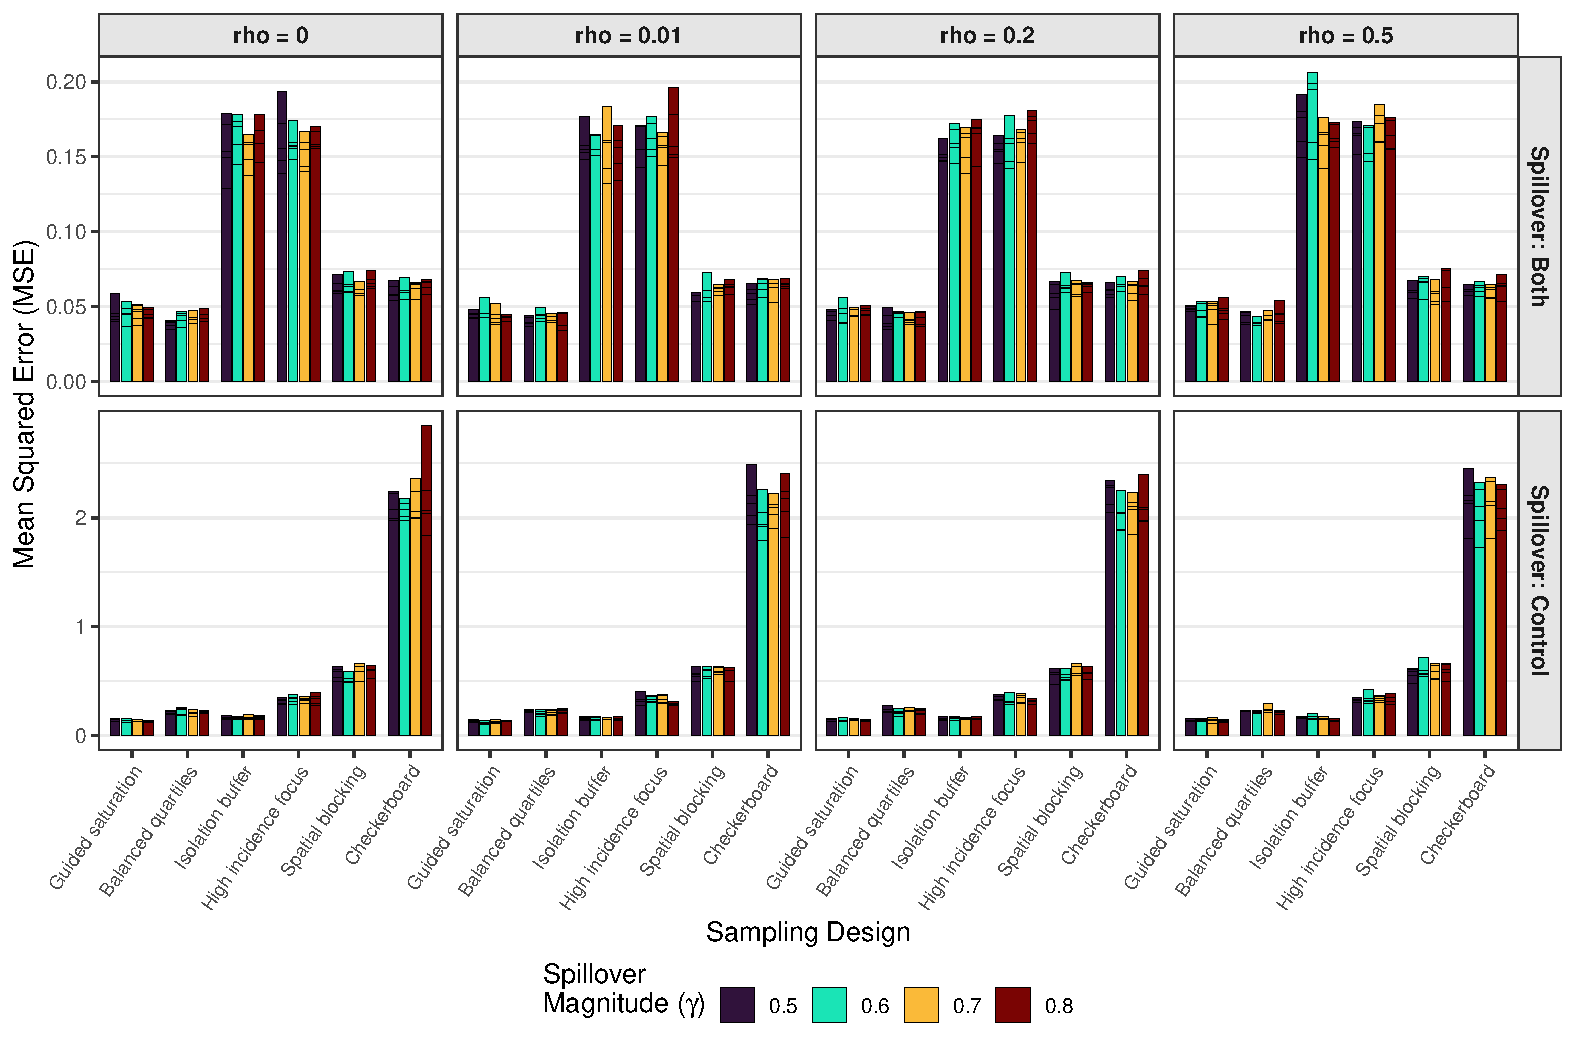
\includegraphics[width=0.98\linewidth,height=0.74\textheight,keepaspectratio]{figures/fig_mse_by_design_6design_queen_journal.pdf}
\caption{Grid MSE at $\tau=1$ under queen contiguity for the detailed six-design subset. Columns show outcome spatial dependence and rows spillover regimes. Bars overlay five incidence configurations, with horizontal lines marking their values; colors show spillover magnitude. Table~\ref{tab:grid-srs} additionally includes plain saturation, Balanced Halves and SRS. Regime scales differ.}\label{fig:grid}
\end{figure*}
}

\newcommand{\CTJMeanFigure}{%
\begin{figure*}[tp]
\centering
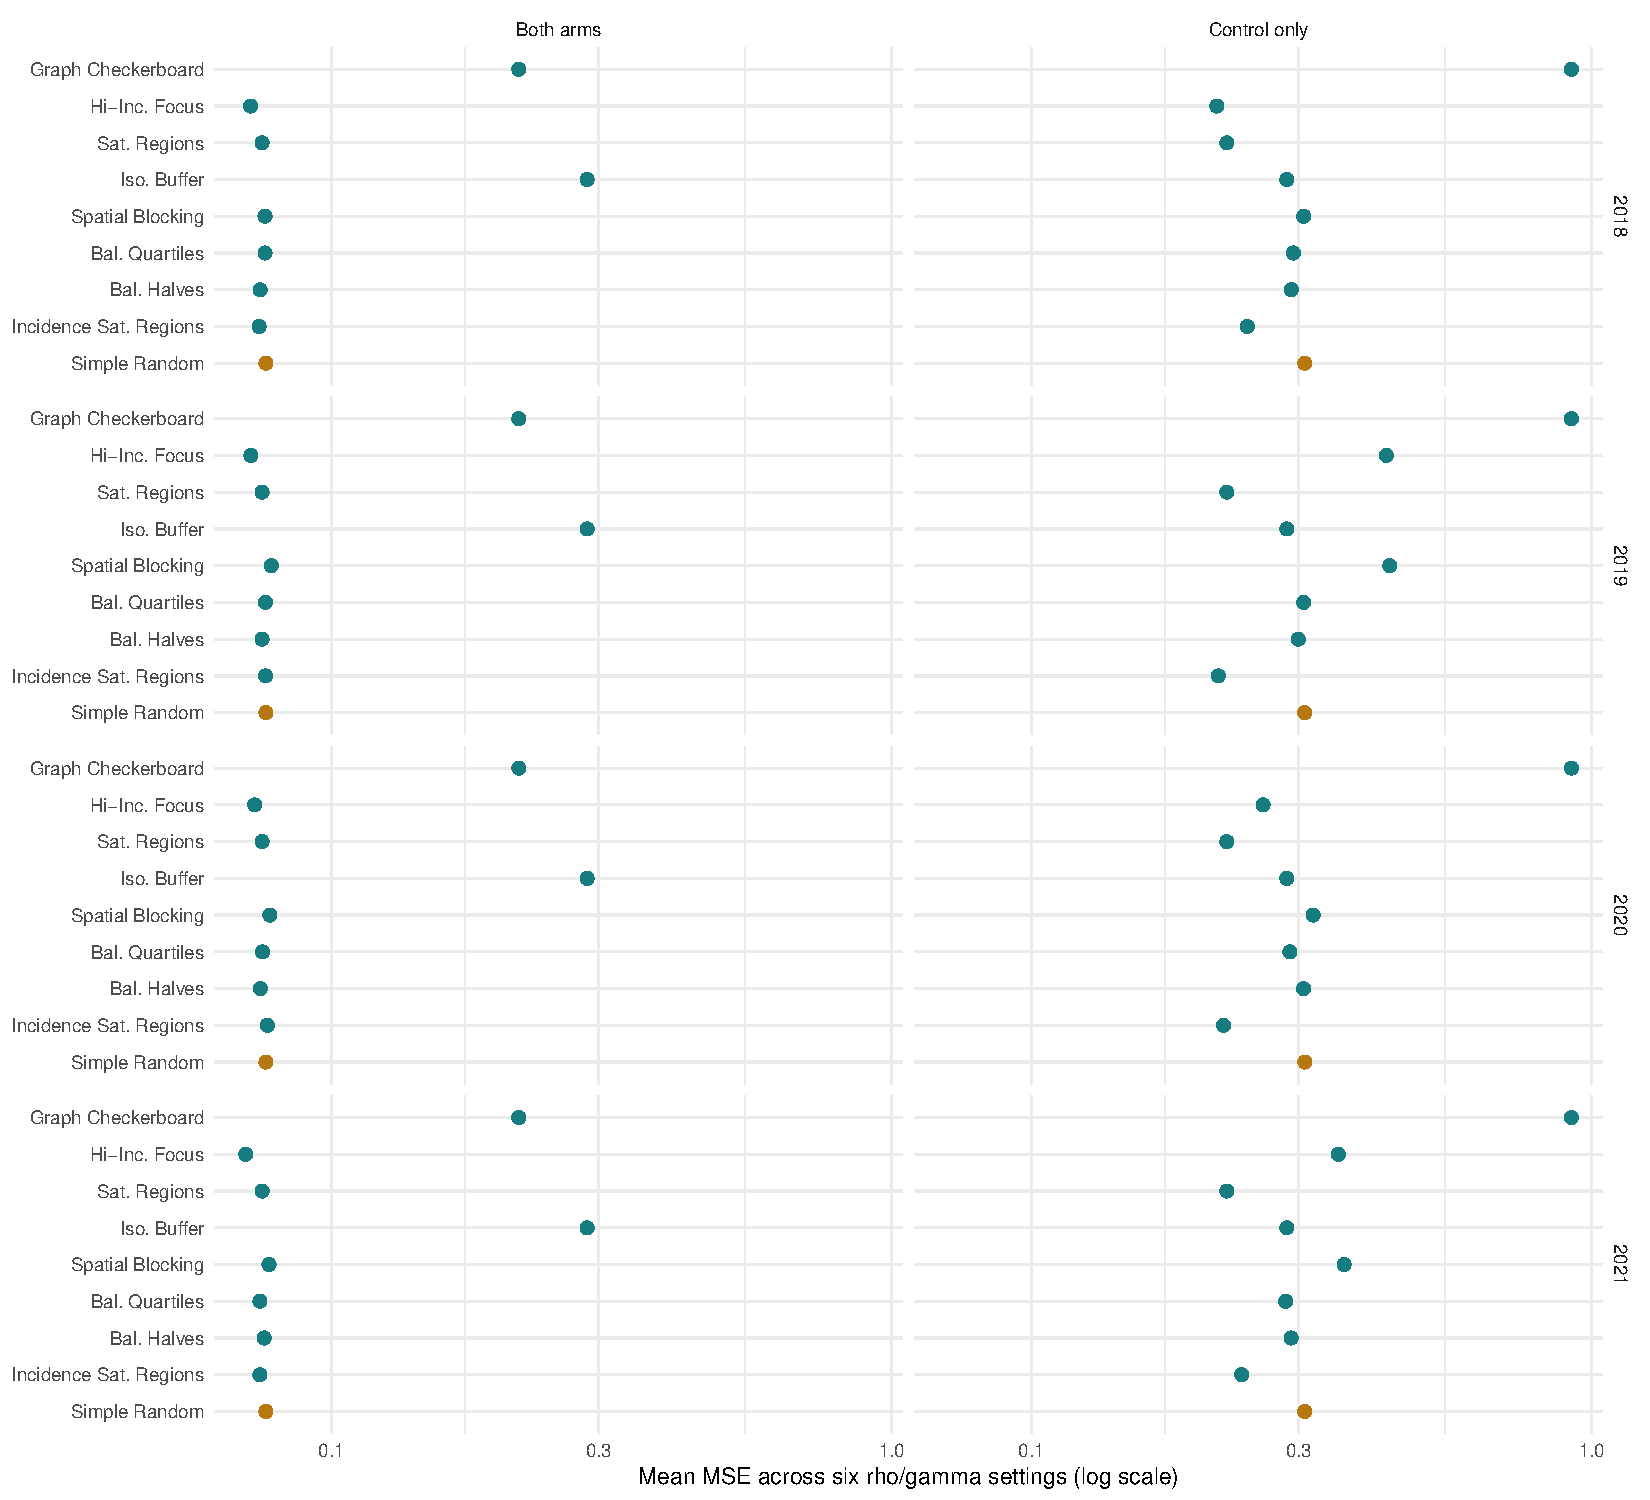
\includegraphics[width=0.98\linewidth,height=0.74\textheight,keepaspectratio]{figures/real_sud/primary_yearly_mse_journal.pdf}
\caption{Completed primary application mean MSE by design, observed planning year and spillover regime, queen weights and education outcome. Each point equally averages six $\rho/\gamma$ pairs on a common logarithmic scale; gold marks SRS. Shared sources repeat across years and are not independent replications. No pooled MC intervals are supplied.}\label{fig:nc-mse}
\end{figure*}
}

\newcommand{\CTJRiskFigure}{%
\begin{figure*}[tp]
\centering
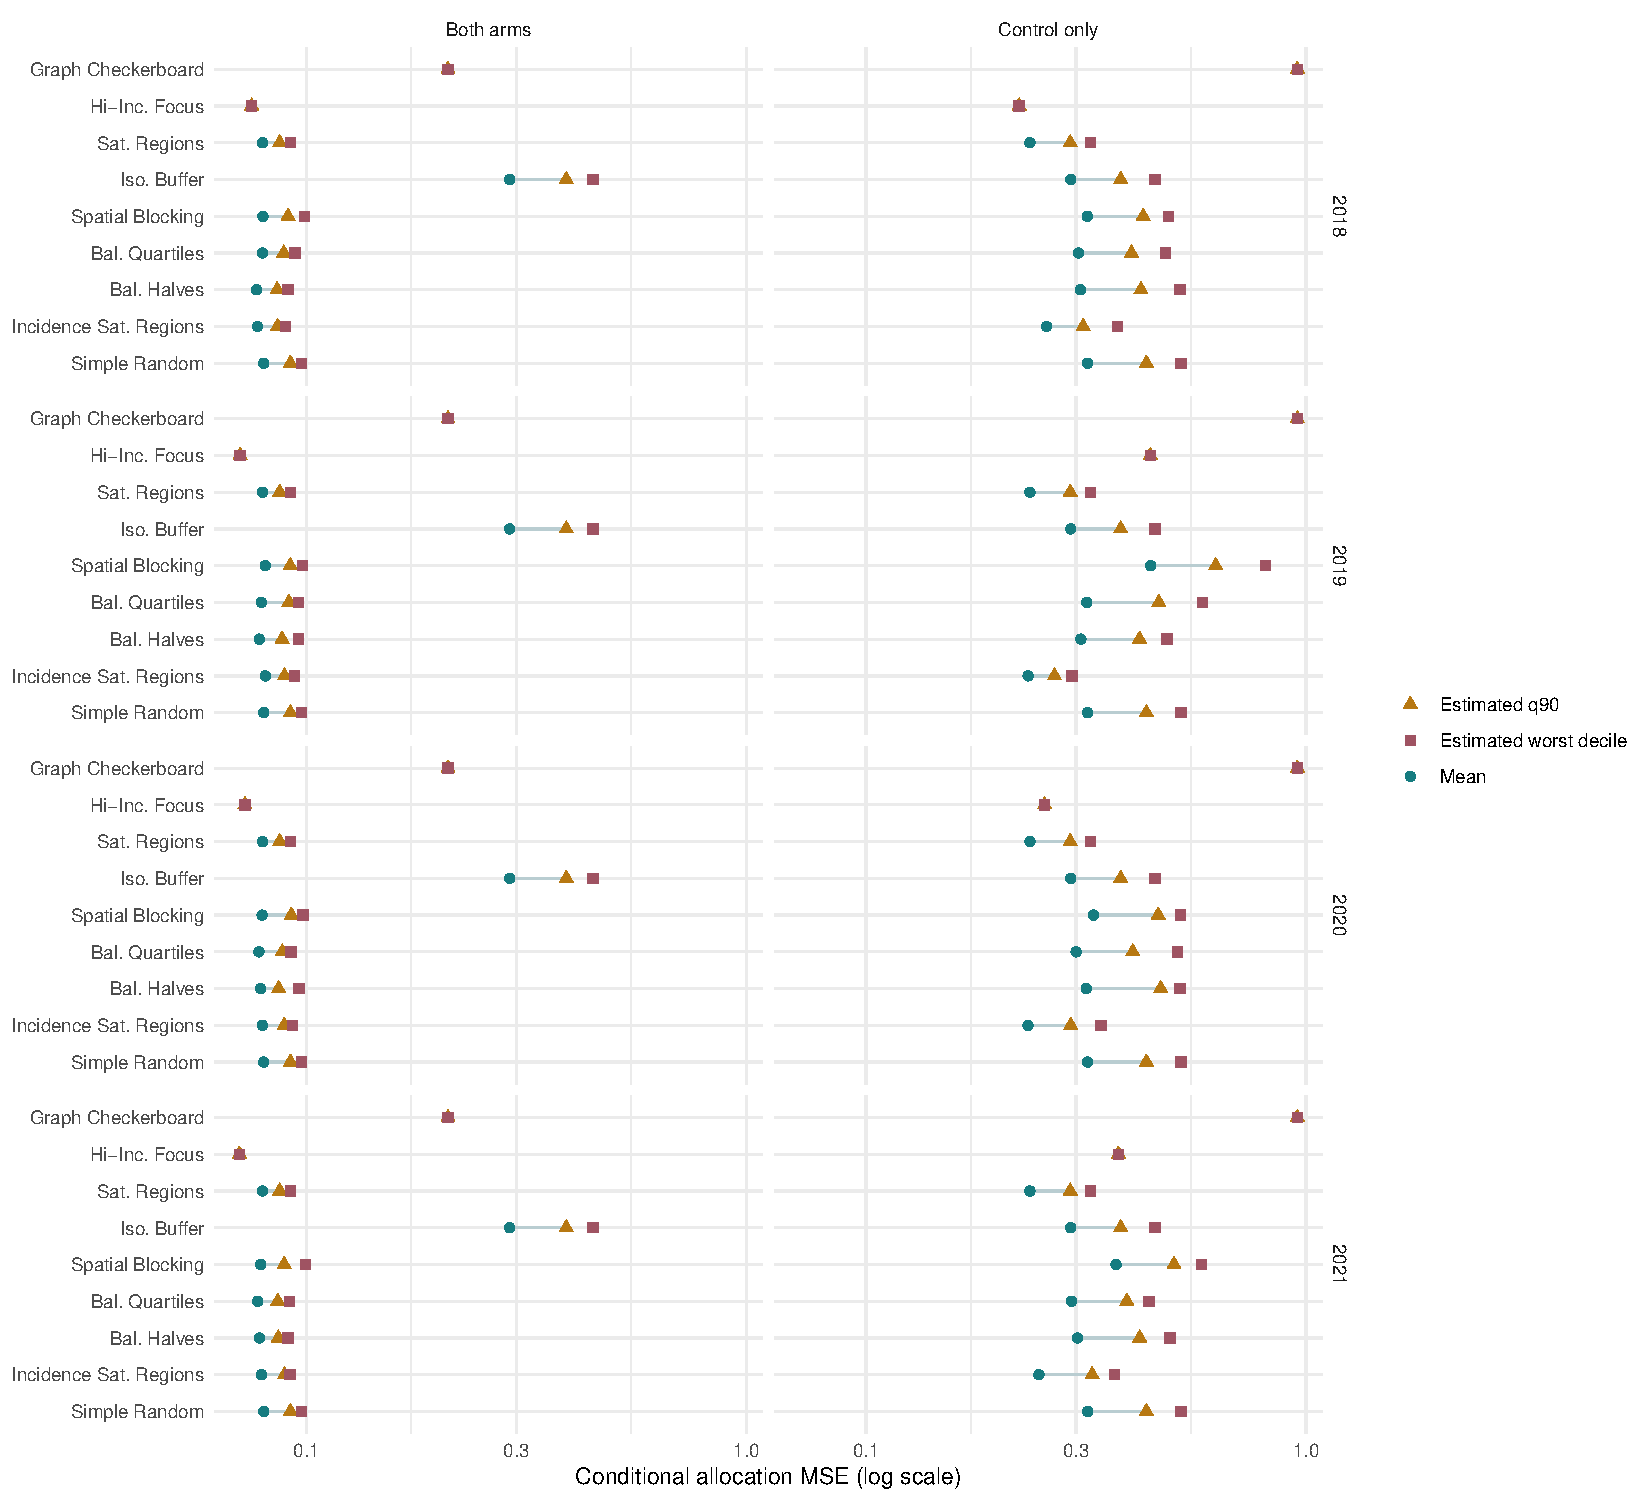
\includegraphics[width=0.98\linewidth,height=0.74\textheight,keepaspectratio]{figures/real_sud/refined_allocation_risk_journal.pdf}
\caption{Refined allocation-risk estimates at primary queen $\rho=0.5,\gamma=0.8$. Mean MSE, estimated allocation q90 and estimated worst-decile mean refer to the same 100 sampled assignments, using 400 outcomes per stochastic assignment or 1,000 for singleton supports. Finite-outcome tails and membership remain uncertain; this extension is not fresh allocation confirmation.}\label{fig:nc-risk}
\end{figure*}
}

\newcommand{\CTJBudgetFigure}{%
\begin{figure*}[tp]
\centering
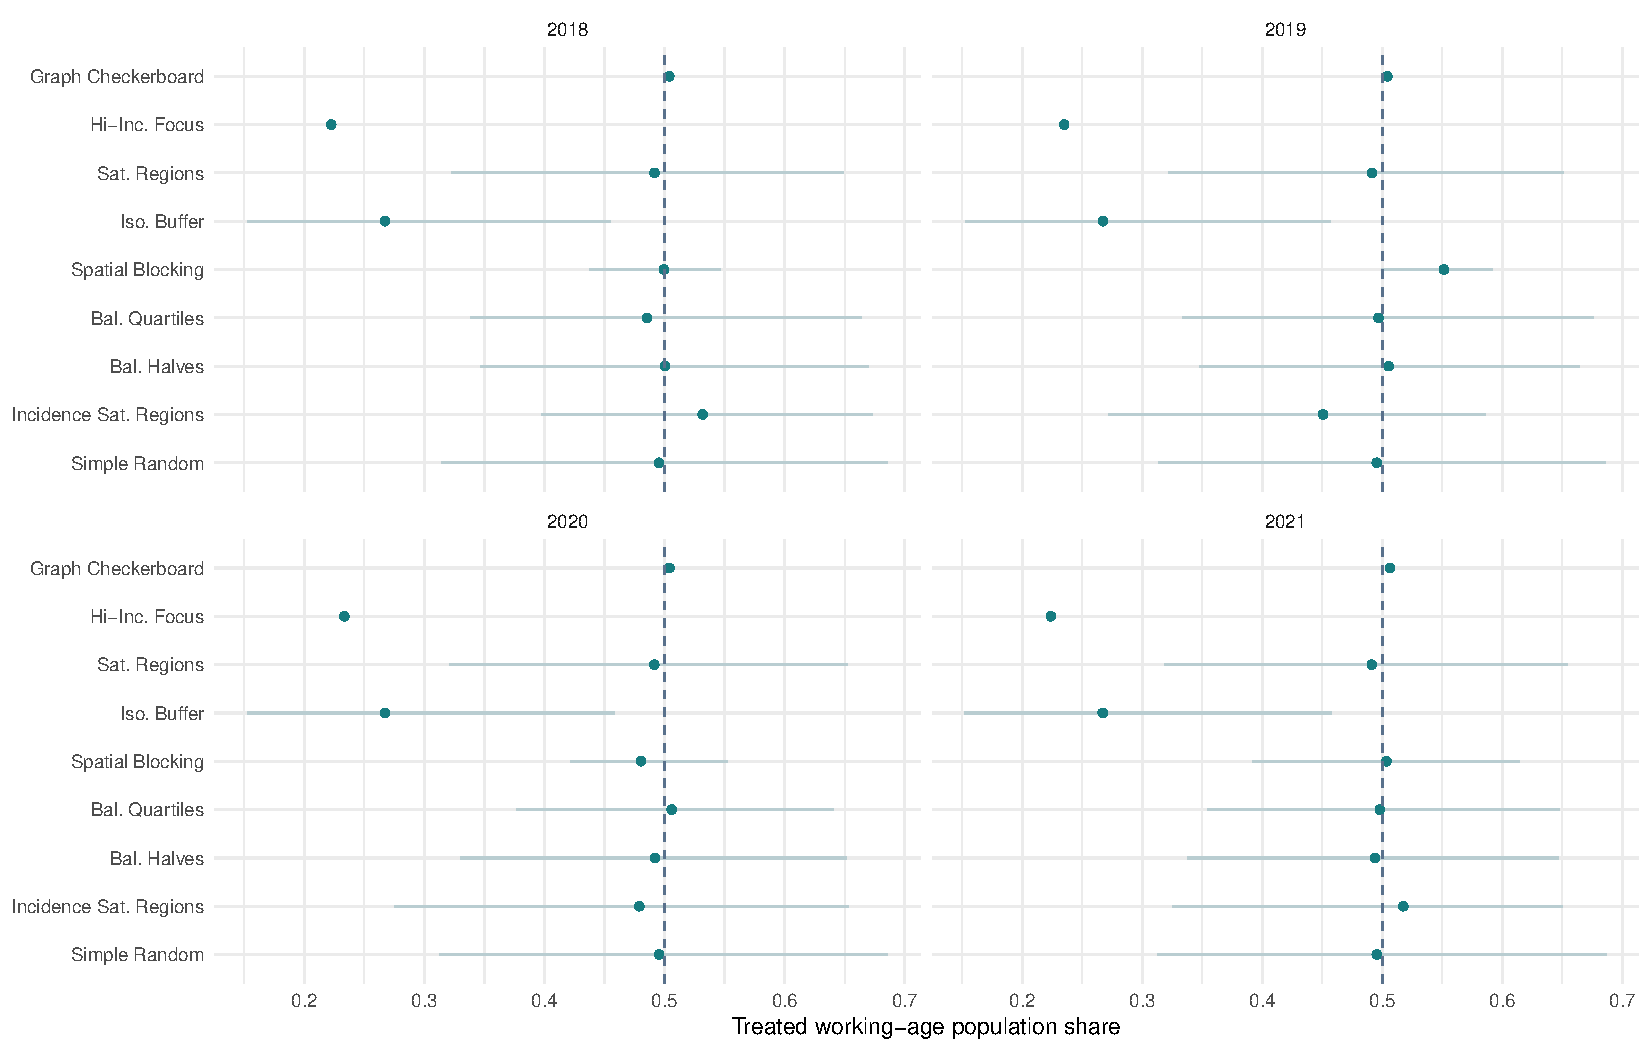
\includegraphics[width=0.98\linewidth,height=0.74\textheight,keepaspectratio]{figures/real_sud/population_shares_journal.pdf}
\caption{Treated annual working-age population shares under primary queen assignments. Points are means and segments show sampled allocation ranges; the dashed line marks 50\%. Budgets use the both-arms run, with allocation support unchanged by regime. Population is geographic reach, not healthcare-professional enrollment or implementation cost.}\label{fig:nc-pop}
\end{figure*}
}
